\documentclass[1p]{elsarticle_modified}
%\bibliographystyle{elsarticle-num}

%\usepackage[colorlinks]{hyperref}
%\usepackage{abbrmath_seonhwa} %\Abb, \Ascr, \Acal ,\Abf, \Afrak
\usepackage{amsfonts}
\usepackage{amssymb}
\usepackage{amsmath}
\usepackage{amsthm}
\usepackage{scalefnt}
\usepackage{amsbsy}
\usepackage{kotex}
\usepackage{caption}
\usepackage{subfig}
\usepackage{color}
\usepackage{graphicx}
\usepackage{xcolor} %% white, black, red, green, blue, cyan, magenta, yellow
\usepackage{float}
\usepackage{setspace}
\usepackage{hyperref}

\usepackage{tikz}
\usetikzlibrary{arrows}

\usepackage{multirow}
\usepackage{array} % fixed length table
\usepackage{hhline}

%%%%%%%%%%%%%%%%%%%%%
\makeatletter
\renewcommand*\env@matrix[1][\arraystretch]{%
	\edef\arraystretch{#1}%
	\hskip -\arraycolsep
	\let\@ifnextchar\new@ifnextchar
	\array{*\c@MaxMatrixCols c}}
\makeatother %https://tex.stackexchange.com/questions/14071/how-can-i-increase-the-line-spacing-in-a-matrix
%%%%%%%%%%%%%%%

\usepackage[normalem]{ulem}

\newcommand{\msout}[1]{\ifmmode\text{\sout{\ensuremath{#1}}}\else\sout{#1}\fi}
%SOURCE: \msout is \stkout macro in https://tex.stackexchange.com/questions/20609/strikeout-in-math-mode

\newcommand{\cancel}[1]{
	\ifmmode
	{\color{red}\msout{#1}}
	\else
	{\color{red}\sout{#1}}
	\fi
}

\newcommand{\add}[1]{
	{\color{blue}\uwave{#1}}
}

\newcommand{\replace}[2]{
	\ifmmode
	{\color{red}\msout{#1}}{\color{blue}\uwave{#2}}
	\else
	{\color{red}\sout{#1}}{\color{blue}\uwave{#2}}
	\fi
}

\newcommand{\Sol}{\mathcal{S}} %segment
\newcommand{\D}{D} %diagram
\newcommand{\A}{\mathcal{A}} %arc


%%%%%%%%%%%%%%%%%%%%%%%%%%%%%5 test

\def\sl{\operatorname{\textup{SL}}(2,\Cbb)}
\def\psl{\operatorname{\textup{PSL}}(2,\Cbb)}
\def\quan{\mkern 1mu \triangleright \mkern 1mu}

\theoremstyle{definition}
\newtheorem{thm}{Theorem}[section]
\newtheorem{prop}[thm]{Proposition}
\newtheorem{lem}[thm]{Lemma}
\newtheorem{ques}[thm]{Question}
\newtheorem{cor}[thm]{Corollary}
\newtheorem{defn}[thm]{Definition}
\newtheorem{exam}[thm]{Example}
\newtheorem{rmk}[thm]{Remark}
\newtheorem{alg}[thm]{Algorithm}

\newcommand{\I}{\sqrt{-1}}
\begin{document}

%\begin{frontmatter}
%
%\title{Boundary parabolic representations of knots up to 8 crossings}
%
%%% Group authors per affiliation:
%\author{Yunhi Cho} 
%\address{Department of Mathematics, University of Seoul, Seoul, Korea}
%\ead{yhcho@uos.ac.kr}
%
%
%\author{Seonhwa Kim} %\fnref{s_kim}}
%\address{Center for Geometry and Physics, Institute for Basic Science, Pohang, 37673, Korea}
%\ead{ryeona17@ibs.re.kr}
%
%\author{Hyuk Kim}
%\address{Department of Mathematical Sciences, Seoul National University, Seoul 08826, Korea}
%\ead{hyukkim@snu.ac.kr}
%
%\author{Seokbeom Yoon}
%\address{Department of Mathematical Sciences, Seoul National University, Seoul, 08826,  Korea}
%\ead{sbyoon15@snu.ac.kr}
%
%\begin{abstract}
%We find all boundary parabolic representation of knots up to 8 crossings.
%
%\end{abstract}
%\begin{keyword}
%    \MSC[2010] 57M25 
%\end{keyword}
%
%\end{frontmatter}

%\linenumbers
%\tableofcontents
%
\newcommand\colored[1]{\textcolor{white}{\rule[-0.35ex]{0.8em}{1.4ex}}\kern-0.8em\color{red} #1}%
%\newcommand\colored[1]{\textcolor{white}{ #1}\kern-2.17ex	\textcolor{white}{ #1}\kern-1.81ex	\textcolor{white}{ #1}\kern-2.15ex\color{red}#1	}

{\Large $\underline{12a_{0529}~(K12a_{0529})}$}

\setlength{\tabcolsep}{10pt}
\renewcommand{\arraystretch}{1.6}
\vspace{1cm}\begin{tabular}{m{100pt}>{\centering\arraybackslash}m{274pt}}
\multirow{5}{120pt}{
	\centering
	\includegraphics[width=112pt]{../../../GIT/diagram.site/Diagrams/png/1330_12a_0529.png}\\
\ \ \ A knot diagram\footnotemark}&
\allowdisplaybreaks
\textbf{Linearized knot diagam} \\
\cline{2-2}
 &
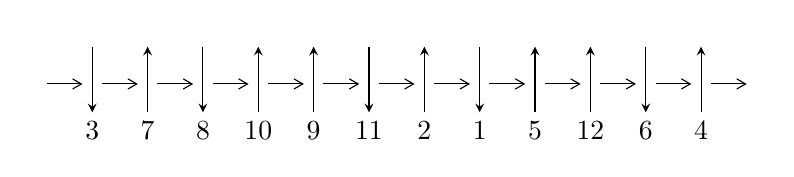
\begin{tikzpicture}[x=20pt, y=17pt]
	% nodes
	\node (C0) at (0, 0) {};
	\node (C1) at (1, 0) {};
	\node (C1U) at (1, +1) {};
	\node (C1D) at (1, -1) {3};

	\node (C2) at (2, 0) {};
	\node (C2U) at (2, +1) {};
	\node (C2D) at (2, -1) {7};

	\node (C3) at (3, 0) {};
	\node (C3U) at (3, +1) {};
	\node (C3D) at (3, -1) {8};

	\node (C4) at (4, 0) {};
	\node (C4U) at (4, +1) {};
	\node (C4D) at (4, -1) {10};

	\node (C5) at (5, 0) {};
	\node (C5U) at (5, +1) {};
	\node (C5D) at (5, -1) {9};

	\node (C6) at (6, 0) {};
	\node (C6U) at (6, +1) {};
	\node (C6D) at (6, -1) {11};

	\node (C7) at (7, 0) {};
	\node (C7U) at (7, +1) {};
	\node (C7D) at (7, -1) {2};

	\node (C8) at (8, 0) {};
	\node (C8U) at (8, +1) {};
	\node (C8D) at (8, -1) {1};

	\node (C9) at (9, 0) {};
	\node (C9U) at (9, +1) {};
	\node (C9D) at (9, -1) {5};

	\node (C10) at (10, 0) {};
	\node (C10U) at (10, +1) {};
	\node (C10D) at (10, -1) {12};

	\node (C11) at (11, 0) {};
	\node (C11U) at (11, +1) {};
	\node (C11D) at (11, -1) {6};

	\node (C12) at (12, 0) {};
	\node (C12U) at (12, +1) {};
	\node (C12D) at (12, -1) {4};
	\node (C13) at (13, 0) {};

	% arrows
	\draw[->,>={angle 60}]
	(C0) edge (C1) (C1) edge (C2) (C2) edge (C3) (C3) edge (C4) (C4) edge (C5) (C5) edge (C6) (C6) edge (C7) (C7) edge (C8) (C8) edge (C9) (C9) edge (C10) (C10) edge (C11) (C11) edge (C12) (C12) edge (C13) ;	\draw[->,>=stealth]
	(C1U) edge (C1D) (C2D) edge (C2U) (C3U) edge (C3D) (C4D) edge (C4U) (C5D) edge (C5U) (C6U) edge (C6D) (C7D) edge (C7U) (C8U) edge (C8D) (C9D) edge (C9U) (C10D) edge (C10U) (C11U) edge (C11D) (C12D) edge (C12U) ;
	\end{tikzpicture} \\
\hhline{~~} \\& 
\textbf{Solving Sequence} \\ \cline{2-2} 
 &
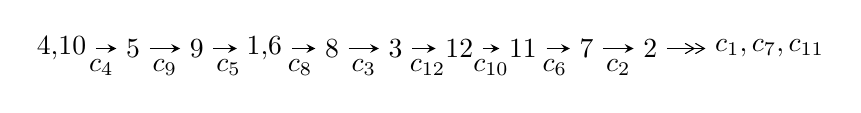
\begin{tikzpicture}[x=23pt, y=7pt]
	% node
	\node (A0) at (-1/8, 0) {4,10};
	\node (A1) at (1, 0) {5};
	\node (A2) at (2, 0) {9};
	\node (A3) at (49/16, 0) {1,6};
	\node (A4) at (33/8, 0) {8};
	\node (A5) at (41/8, 0) {3};
	\node (A6) at (49/8, 0) {12};
	\node (A7) at (57/8, 0) {11};
	\node (A8) at (65/8, 0) {7};
	\node (A9) at (73/8, 0) {2};
	\node (C1) at (1/2, -1) {$c_{4}$};
	\node (C2) at (3/2, -1) {$c_{9}$};
	\node (C3) at (5/2, -1) {$c_{5}$};
	\node (C4) at (29/8, -1) {$c_{8}$};
	\node (C5) at (37/8, -1) {$c_{3}$};
	\node (C6) at (45/8, -1) {$c_{12}$};
	\node (C7) at (53/8, -1) {$c_{10}$};
	\node (C8) at (61/8, -1) {$c_{6}$};
	\node (C9) at (69/8, -1) {$c_{2}$};
	\node (A10) at (11, 0) {$c_{1},c_{7},c_{11}$};

	% edge
	\draw[->,>=stealth]	
	(A0) edge (A1) (A1) edge (A2) (A2) edge (A3) (A3) edge (A4) (A4) edge (A5) (A5) edge (A6) (A6) edge (A7) (A7) edge (A8) (A8) edge (A9) ;
	\draw[->>,>={angle 60}]	
	(A9) edge (A10);
\end{tikzpicture} \\ 

\end{tabular} \\

\footnotetext{
The image of knot diagram is generated by the software ``\textbf{Draw programme}" developed by Andrew Bartholomew(\url{http://www.layer8.co.uk/maths/draw/index.htm\#Running-draw}), where we modified some parts for our purpose(\url{https://github.com/CATsTAILs/LinksPainter}).
}\phantom \\ \newline 
\centering \textbf{Ideals for irreducible components\footnotemark of $X_{\text{par}}$} 
 
\begin{align*}
I^u_{1}&=\langle 
-3.53233\times10^{65} u^{75}+2.53432\times10^{65} u^{74}+\cdots+3.87343\times10^{66} b+4.07069\times10^{67},\\
\phantom{I^u_{1}}&\phantom{= \langle  }-6.56457\times10^{66} u^{75}+6.09413\times10^{66} u^{74}+\cdots+6.58484\times10^{67} a+8.05766\times10^{68},\\
\phantom{I^u_{1}}&\phantom{= \langle  }u^{76}- u^{75}+\cdots-158 u+17\rangle \\
I^u_{2}&=\langle 
- u^3+b- u,\;- u^3+a,\;u^{12}+4 u^{10}+6 u^8+5 u^6+3 u^4- u^3+u^2- u+1\rangle \\
I^u_{3}&=\langle 
b- a- u,\;a^6+6 a^5 u+a^5+5 a^4 u-16 a^4-24 a^3 u-12 a^3-16 a^2 u+21 a^2+10 a u+12 a+4 u-1,\;u^2+1\rangle \\
I^u_{4}&=\langle 
- u^3+b- u,\;- u^3+a,\;u^{18}+6 u^{16}+\cdots+2 u+1\rangle \\
\\
\end{align*}
\raggedright * 4 irreducible components of $\dim_{\mathbb{C}}=0$, with total 118 representations.\\
\footnotetext{All coefficients of polynomials are rational numbers. But the coefficients are sometimes approximated in decimal forms when there is not enough margin.}
\newpage
\renewcommand{\arraystretch}{1}
\centering \section*{I. $I^u_{1}= \langle -3.53\times10^{65} u^{75}+2.53\times10^{65} u^{74}+\cdots+3.87\times10^{66} b+4.07\times10^{67},\;-6.56\times10^{66} u^{75}+6.09\times10^{66} u^{74}+\cdots+6.58\times10^{67} a+8.06\times10^{68},\;u^{76}- u^{75}+\cdots-158 u+17 \rangle$}
\flushleft \textbf{(i) Arc colorings}\\
\begin{tabular}{m{7pt} m{180pt} m{7pt} m{180pt} }
\flushright $a_{4}=$&$\begin{pmatrix}1\\0\end{pmatrix}$ \\
\flushright $a_{10}=$&$\begin{pmatrix}0\\u\end{pmatrix}$ \\
\flushright $a_{5}=$&$\begin{pmatrix}1\\- u^2\end{pmatrix}$ \\
\flushright $a_{9}=$&$\begin{pmatrix}- u\\u^3+u\end{pmatrix}$ \\
\flushright $a_{1}=$&$\begin{pmatrix}0.0996921 u^{75}-0.0925479 u^{74}+\cdots+85.8969 u-12.2367\\0.0911937 u^{75}-0.0654283 u^{74}+\cdots+51.1583 u-10.5093\end{pmatrix}$ \\
\flushright $a_{6}=$&$\begin{pmatrix}u^2+1\\- u^4-2 u^2\end{pmatrix}$ \\
\flushright $a_{8}=$&$\begin{pmatrix}0.600810 u^{75}-0.591223 u^{74}+\cdots+251.305 u-43.7031\\0.257472 u^{75}-0.267396 u^{74}+\cdots+57.0402 u-9.17170\end{pmatrix}$ \\
\flushright $a_{3}=$&$\begin{pmatrix}0.723306 u^{75}-0.563802 u^{74}+\cdots+284.437 u-45.2027\\0.217757 u^{75}-0.0902812 u^{74}+\cdots+78.2752 u-11.1735\end{pmatrix}$ \\
\flushright $a_{12}=$&$\begin{pmatrix}0.00849846 u^{75}-0.0271196 u^{74}+\cdots+34.7387 u-1.72742\\0.0911937 u^{75}-0.0654283 u^{74}+\cdots+51.1583 u-10.5093\end{pmatrix}$ \\
\flushright $a_{11}=$&$\begin{pmatrix}0.0993703 u^{75}-0.0950018 u^{74}+\cdots+84.3319 u-12.4324\\0.124410 u^{75}-0.0564865 u^{74}+\cdots+53.1573 u-10.4350\end{pmatrix}$ \\
\flushright $a_{7}=$&$\begin{pmatrix}0.625336 u^{75}-0.501248 u^{74}+\cdots+242.513 u-48.2108\\-0.0722923 u^{75}+0.0771458 u^{74}+\cdots-12.4899 u+3.80427\end{pmatrix}$ \\
\flushright $a_{2}=$&$\begin{pmatrix}1.62071 u^{75}-1.09263 u^{74}+\cdots+534.442 u-76.5897\\0.191754 u^{75}-0.0384194 u^{74}+\cdots+32.9728 u-7.14572\end{pmatrix}$\\&\end{tabular}
\flushleft \textbf{(ii) Obstruction class $= -1$}\\~\\
\flushleft \textbf{(iii) Cusp Shapes $= -0.569931 u^{75}+0.359505 u^{74}+\cdots-304.744 u+50.6300$}\\~\\
\newpage\renewcommand{\arraystretch}{1}
\flushleft \textbf{(iv) u-Polynomials at the component}\newline \\
\begin{tabular}{m{50pt}|m{274pt}}
Crossings & \hspace{64pt}u-Polynomials at each crossing \\
\hline $$\begin{aligned}c_{1}\end{aligned}$$&$\begin{aligned}
&u^{76}+36 u^{75}+\cdots+19 u+4
\end{aligned}$\\
\hline $$\begin{aligned}c_{2},c_{7}\end{aligned}$$&$\begin{aligned}
&u^{76}-2 u^{75}+\cdots-5 u+2
\end{aligned}$\\
\hline $$\begin{aligned}c_{3}\end{aligned}$$&$\begin{aligned}
&u^{76}+2 u^{75}+\cdots-1177 u+202
\end{aligned}$\\
\hline $$\begin{aligned}c_{4},c_{5},c_{9}\end{aligned}$$&$\begin{aligned}
&u^{76}- u^{75}+\cdots-158 u+17
\end{aligned}$\\
\hline $$\begin{aligned}c_{6},c_{11}\end{aligned}$$&$\begin{aligned}
&u^{76}- u^{75}+\cdots-100 u+17
\end{aligned}$\\
\hline $$\begin{aligned}c_{8}\end{aligned}$$&$\begin{aligned}
&u^{76}-10 u^{75}+\cdots-18835 u+1862
\end{aligned}$\\
\hline $$\begin{aligned}c_{10}\end{aligned}$$&$\begin{aligned}
&u^{76}-29 u^{75}+\cdots-3906 u+289
\end{aligned}$\\
\hline $$\begin{aligned}c_{12}\end{aligned}$$&$\begin{aligned}
&u^{76}+8 u^{75}+\cdots+1172713 u+156832
\end{aligned}$\\
\hline
\end{tabular}\\~\\
\newpage\renewcommand{\arraystretch}{1}
\flushleft \textbf{(v) Riley Polynomials at the component}\newline \\
\begin{tabular}{m{50pt}|m{274pt}}
Crossings & \hspace{64pt}Riley Polynomials at each crossing \\
\hline $$\begin{aligned}c_{1}\end{aligned}$$&$\begin{aligned}
&y^{76}+8 y^{75}+\cdots+191 y+16
\end{aligned}$\\
\hline $$\begin{aligned}c_{2},c_{7}\end{aligned}$$&$\begin{aligned}
&y^{76}+36 y^{75}+\cdots+19 y+4
\end{aligned}$\\
\hline $$\begin{aligned}c_{3}\end{aligned}$$&$\begin{aligned}
&y^{76}-20 y^{75}+\cdots-1880229 y+40804
\end{aligned}$\\
\hline $$\begin{aligned}c_{4},c_{5},c_{9}\end{aligned}$$&$\begin{aligned}
&y^{76}+81 y^{75}+\cdots-13438 y+289
\end{aligned}$\\
\hline $$\begin{aligned}c_{6},c_{11}\end{aligned}$$&$\begin{aligned}
&y^{76}+29 y^{75}+\cdots+3906 y+289
\end{aligned}$\\
\hline $$\begin{aligned}c_{8}\end{aligned}$$&$\begin{aligned}
&y^{76}+12 y^{75}+\cdots+54812019 y+3467044
\end{aligned}$\\
\hline $$\begin{aligned}c_{10}\end{aligned}$$&$\begin{aligned}
&y^{76}+49 y^{75}+\cdots+20899954 y+83521
\end{aligned}$\\
\hline $$\begin{aligned}c_{12}\end{aligned}$$&$\begin{aligned}
&y^{76}+24 y^{75}+\cdots+1500857096879 y+24596276224
\end{aligned}$\\
\hline
\end{tabular}\\~\\
\newpage\flushleft \textbf{(vi) Complex Volumes and Cusp Shapes}
$$\begin{array}{c|c|c}  
\text{Solutions to }I^u_{1}& \I (\text{vol} + \sqrt{-1}CS) & \text{Cusp shape}\\
 \hline 
\begin{aligned}
u &= \phantom{-}0.871703 + 0.337657 I \\
a &= \phantom{-}0.531191 - 0.397620 I \\
b &= -0.72291 - 1.41153 I\end{aligned}
 & -0.96411 + 12.75580 I & \phantom{-0.000000 } 0 \\ \hline\begin{aligned}
u &= \phantom{-}0.871703 - 0.337657 I \\
a &= \phantom{-}0.531191 + 0.397620 I \\
b &= -0.72291 + 1.41153 I\end{aligned}
 & -0.96411 - 12.75580 I & \phantom{-0.000000 } 0 \\ \hline\begin{aligned}
u &= -0.341605 + 0.864408 I \\
a &= -0.850996 + 0.602062 I \\
b &= -0.568836 + 0.390828 I\end{aligned}
 & -2.34126 - 6.14169 I & \phantom{-0.000000 } 0 \\ \hline\begin{aligned}
u &= -0.341605 - 0.864408 I \\
a &= -0.850996 - 0.602062 I \\
b &= -0.568836 - 0.390828 I\end{aligned}
 & -2.34126 + 6.14169 I & \phantom{-0.000000 } 0 \\ \hline\begin{aligned}
u &= -0.154405 + 0.907290 I \\
a &= -0.406956 + 0.726577 I \\
b &= -0.308364 + 0.691108 I\end{aligned}
 & -3.62597 + 0.74459 I & \phantom{-0.000000 } 0 \\ \hline\begin{aligned}
u &= -0.154405 - 0.907290 I \\
a &= -0.406956 - 0.726577 I \\
b &= -0.308364 - 0.691108 I\end{aligned}
 & -3.62597 - 0.74459 I & \phantom{-0.000000 } 0 \\ \hline\begin{aligned}
u &= \phantom{-}0.835900 + 0.374263 I \\
a &= \phantom{-}0.683754 - 0.340500 I \\
b &= -0.536338 - 1.288420 I\end{aligned}
 & -3.08946 + 4.96821 I & \phantom{-0.000000 } 0 \\ \hline\begin{aligned}
u &= \phantom{-}0.835900 - 0.374263 I \\
a &= \phantom{-}0.683754 + 0.340500 I \\
b &= -0.536338 + 1.288420 I\end{aligned}
 & -3.08946 - 4.96821 I & \phantom{-0.000000 } 0 \\ \hline\begin{aligned}
u &= -0.850183 + 0.331328 I \\
a &= -0.543534 - 0.324415 I \\
b &= \phantom{-}0.72960 - 1.31268 I\end{aligned}
 & \phantom{-}1.39164 - 7.76709 I & \phantom{-0.000000 } 0 \\ \hline\begin{aligned}
u &= -0.850183 - 0.331328 I \\
a &= -0.543534 + 0.324415 I \\
b &= \phantom{-}0.72960 + 1.31268 I\end{aligned}
 & \phantom{-}1.39164 + 7.76709 I & \phantom{-0.000000 } 0\\
 \hline 
 \end{array}$$\newpage$$\begin{array}{c|c|c}  
\text{Solutions to }I^u_{1}& \I (\text{vol} + \sqrt{-1}CS) & \text{Cusp shape}\\
 \hline 
\begin{aligned}
u &= -0.742033 + 0.489974 I \\
a &= -1.023820 - 0.198435 I \\
b &= \phantom{-}0.045626 - 0.959753 I\end{aligned}
 & -4.05338 - 4.76438 I & \phantom{-0.000000 -}0. + 6.53613 I \\ \hline\begin{aligned}
u &= -0.742033 - 0.489974 I \\
a &= -1.023820 + 0.198435 I \\
b &= \phantom{-}0.045626 + 0.959753 I\end{aligned}
 & -4.05338 + 4.76438 I & \phantom{-0.000000 } 0. - 6.53613 I \\ \hline\begin{aligned}
u &= -0.682242 + 0.569438 I \\
a &= -1.158730 - 0.084714 I \\
b &= -0.222157 - 0.733705 I\end{aligned}
 & -2.82768 + 2.89502 I & \phantom{-0.000000 } 0 \\ \hline\begin{aligned}
u &= -0.682242 - 0.569438 I \\
a &= -1.158730 + 0.084714 I \\
b &= -0.222157 + 0.733705 I\end{aligned}
 & -2.82768 - 2.89502 I & \phantom{-0.000000 } 0 \\ \hline\begin{aligned}
u &= -0.789625 + 0.287686 I \\
a &= -0.527894 - 0.089515 I \\
b &= \phantom{-}0.842261 - 1.020140 I\end{aligned}
 & \phantom{-}2.89325 - 5.78254 I & \phantom{-}6.56857 + 7.64192 I \\ \hline\begin{aligned}
u &= -0.789625 - 0.287686 I \\
a &= -0.527894 + 0.089515 I \\
b &= \phantom{-}0.842261 + 1.020140 I\end{aligned}
 & \phantom{-}2.89325 + 5.78254 I & \phantom{-}6.56857 - 7.64192 I \\ \hline\begin{aligned}
u &= \phantom{-}0.648168 + 0.502376 I \\
a &= \phantom{-}1.058750 - 0.048900 I \\
b &= -0.003990 - 0.637730 I\end{aligned}
 & -0.33883 + 1.60186 I & \phantom{-}1.60546 - 3.53406 I \\ \hline\begin{aligned}
u &= \phantom{-}0.648168 - 0.502376 I \\
a &= \phantom{-}1.058750 + 0.048900 I \\
b &= -0.003990 + 0.637730 I\end{aligned}
 & -0.33883 - 1.60186 I & \phantom{-}1.60546 + 3.53406 I \\ \hline\begin{aligned}
u &= \phantom{-}0.296301 + 0.763935 I \\
a &= \phantom{-}0.741212 + 0.381539 I \\
b &= \phantom{-}0.358971 + 0.318208 I\end{aligned}
 & -0.23116 + 1.74291 I & -0.33130 - 4.94390 I \\ \hline\begin{aligned}
u &= \phantom{-}0.296301 - 0.763935 I \\
a &= \phantom{-}0.741212 - 0.381539 I \\
b &= \phantom{-}0.358971 - 0.318208 I\end{aligned}
 & -0.23116 - 1.74291 I & -0.33130 + 4.94390 I\\
 \hline 
 \end{array}$$\newpage$$\begin{array}{c|c|c}  
\text{Solutions to }I^u_{1}& \I (\text{vol} + \sqrt{-1}CS) & \text{Cusp shape}\\
 \hline 
\begin{aligned}
u &= \phantom{-}0.737315 + 0.251878 I \\
a &= \phantom{-}0.553553 + 0.102566 I \\
b &= -0.910825 - 0.780758 I\end{aligned}
 & \phantom{-}2.01584 + 1.14854 I & \phantom{-}5.44751 - 1.47076 I \\ \hline\begin{aligned}
u &= \phantom{-}0.737315 - 0.251878 I \\
a &= \phantom{-}0.553553 - 0.102566 I \\
b &= -0.910825 + 0.780758 I\end{aligned}
 & \phantom{-}2.01584 - 1.14854 I & \phantom{-}5.44751 + 1.47076 I \\ \hline\begin{aligned}
u &= \phantom{-}0.075673 + 1.290750 I \\
a &= -0.992398 + 0.464694 I \\
b &= -1.59071 + 0.73360 I\end{aligned}
 & -1.73230 - 4.32456 I & \phantom{-0.000000 } 0 \\ \hline\begin{aligned}
u &= \phantom{-}0.075673 - 1.290750 I \\
a &= -0.992398 - 0.464694 I \\
b &= -1.59071 - 0.73360 I\end{aligned}
 & -1.73230 + 4.32456 I & \phantom{-0.000000 } 0 \\ \hline\begin{aligned}
u &= -0.096475 + 1.302650 I \\
a &= \phantom{-}0.965712 + 0.242844 I \\
b &= \phantom{-}1.61430 + 0.52832 I\end{aligned}
 & \phantom{-}0.119164 - 0.754172 I & \phantom{-0.000000 } 0 \\ \hline\begin{aligned}
u &= -0.096475 - 1.302650 I \\
a &= \phantom{-}0.965712 - 0.242844 I \\
b &= \phantom{-}1.61430 - 0.52832 I\end{aligned}
 & \phantom{-}0.119164 + 0.754172 I & \phantom{-0.000000 } 0 \\ \hline\begin{aligned}
u &= -0.147580 + 1.317830 I \\
a &= \phantom{-}0.943837 - 0.268717 I \\
b &= \phantom{-}1.69097 + 0.06926 I\end{aligned}
 & \phantom{-}0.41502 - 3.35037 I & \phantom{-0.000000 } 0 \\ \hline\begin{aligned}
u &= -0.147580 - 1.317830 I \\
a &= \phantom{-}0.943837 + 0.268717 I \\
b &= \phantom{-}1.69097 - 0.06926 I\end{aligned}
 & \phantom{-}0.41502 + 3.35037 I & \phantom{-0.000000 } 0 \\ \hline\begin{aligned}
u &= \phantom{-}0.172897 + 1.322130 I \\
a &= -0.933142 - 0.519121 I \\
b &= -1.72379 - 0.15408 I\end{aligned}
 & -1.15919 + 8.40041 I & \phantom{-0.000000 } 0 \\ \hline\begin{aligned}
u &= \phantom{-}0.172897 - 1.322130 I \\
a &= -0.933142 + 0.519121 I \\
b &= -1.72379 + 0.15408 I\end{aligned}
 & -1.15919 - 8.40041 I & \phantom{-0.000000 } 0\\
 \hline 
 \end{array}$$\newpage$$\begin{array}{c|c|c}  
\text{Solutions to }I^u_{1}& \I (\text{vol} + \sqrt{-1}CS) & \text{Cusp shape}\\
 \hline 
\begin{aligned}
u &= \phantom{-}0.096112 + 1.369190 I \\
a &= -0.414099 + 0.096497 I \\
b &= -1.162900 + 0.290588 I\end{aligned}
 & -4.86388 + 2.38505 I & \phantom{-0.000000 } 0 \\ \hline\begin{aligned}
u &= \phantom{-}0.096112 - 1.369190 I \\
a &= -0.414099 - 0.096497 I \\
b &= -1.162900 - 0.290588 I\end{aligned}
 & -4.86388 - 2.38505 I & \phantom{-0.000000 } 0 \\ \hline\begin{aligned}
u &= \phantom{-}0.574787 + 0.059330 I \\
a &= \phantom{-}0.755800 + 1.027700 I \\
b &= -1.230110 + 0.059628 I\end{aligned}
 & \phantom{-}3.16394 + 5.76384 I & \phantom{-}7.59245 - 6.65665 I \\ \hline\begin{aligned}
u &= \phantom{-}0.574787 - 0.059330 I \\
a &= \phantom{-}0.755800 - 1.027700 I \\
b &= -1.230110 - 0.059628 I\end{aligned}
 & \phantom{-}3.16394 - 5.76384 I & \phantom{-}7.59245 + 6.65665 I \\ \hline\begin{aligned}
u &= -0.15045 + 1.41553 I \\
a &= -0.03804 + 1.43925 I \\
b &= -0.619065 + 1.211410 I\end{aligned}
 & -5.22619 + 0.59013 I & \phantom{-0.000000 } 0 \\ \hline\begin{aligned}
u &= -0.15045 - 1.41553 I \\
a &= -0.03804 - 1.43925 I \\
b &= -0.619065 - 1.211410 I\end{aligned}
 & -5.22619 - 0.59013 I & \phantom{-0.000000 } 0 \\ \hline\begin{aligned}
u &= \phantom{-}0.19788 + 1.43555 I \\
a &= \phantom{-}0.03726 + 1.65451 I \\
b &= \phantom{-}0.61403 + 1.34363 I\end{aligned}
 & -4.71578 + 4.11924 I & \phantom{-0.000000 } 0 \\ \hline\begin{aligned}
u &= \phantom{-}0.19788 - 1.43555 I \\
a &= \phantom{-}0.03726 - 1.65451 I \\
b &= \phantom{-}0.61403 - 1.34363 I\end{aligned}
 & -4.71578 - 4.11924 I & \phantom{-0.000000 } 0 \\ \hline\begin{aligned}
u &= \phantom{-}0.28500 + 1.42398 I \\
a &= -0.01702 - 1.54807 I \\
b &= -1.07658 - 1.19558 I\end{aligned}
 & -3.37812 + 4.85193 I & \phantom{-0.000000 } 0 \\ \hline\begin{aligned}
u &= \phantom{-}0.28500 - 1.42398 I \\
a &= -0.01702 + 1.54807 I \\
b &= -1.07658 + 1.19558 I\end{aligned}
 & -3.37812 - 4.85193 I & \phantom{-0.000000 } 0\\
 \hline 
 \end{array}$$\newpage$$\begin{array}{c|c|c}  
\text{Solutions to }I^u_{1}& \I (\text{vol} + \sqrt{-1}CS) & \text{Cusp shape}\\
 \hline 
\begin{aligned}
u &= \phantom{-}0.278329 + 0.467042 I \\
a &= \phantom{-}0.924246 - 0.203547 I \\
b &= -0.054022 + 0.191619 I\end{aligned}
 & \phantom{-}0.259106 + 1.284090 I & \phantom{-}2.32882 - 5.74974 I \\ \hline\begin{aligned}
u &= \phantom{-}0.278329 - 0.467042 I \\
a &= \phantom{-}0.924246 + 0.203547 I \\
b &= -0.054022 - 0.191619 I\end{aligned}
 & \phantom{-}0.259106 - 1.284090 I & \phantom{-}2.32882 + 5.74974 I \\ \hline\begin{aligned}
u &= -0.30726 + 1.43756 I \\
a &= -0.10602 - 1.73731 I \\
b &= \phantom{-}0.99502 - 1.37945 I\end{aligned}
 & -2.64476 - 9.75402 I & \phantom{-0.000000 } 0 \\ \hline\begin{aligned}
u &= -0.30726 - 1.43756 I \\
a &= -0.10602 + 1.73731 I \\
b &= \phantom{-}0.99502 + 1.37945 I\end{aligned}
 & -2.64476 + 9.75402 I & \phantom{-0.000000 } 0 \\ \hline\begin{aligned}
u &= -0.512415 + 0.037742 I \\
a &= -1.03347 + 1.23529 I \\
b &= \phantom{-}1.150490 + 0.265747 I\end{aligned}
 & \phantom{-}4.65569 - 1.02094 I & \phantom{-}10.89176 + 0.78170 I \\ \hline\begin{aligned}
u &= -0.512415 - 0.037742 I \\
a &= -1.03347 - 1.23529 I \\
b &= \phantom{-}1.150490 - 0.265747 I\end{aligned}
 & \phantom{-}4.65569 + 1.02094 I & \phantom{-}10.89176 - 0.78170 I \\ \hline\begin{aligned}
u &= -0.33234 + 1.46432 I \\
a &= -0.34154 - 1.94756 I \\
b &= \phantom{-}0.81603 - 1.59781 I\end{aligned}
 & -4.37511 - 12.05130 I & \phantom{-0.000000 } 0 \\ \hline\begin{aligned}
u &= -0.33234 - 1.46432 I \\
a &= -0.34154 + 1.94756 I \\
b &= \phantom{-}0.81603 + 1.59781 I\end{aligned}
 & -4.37511 + 12.05130 I & \phantom{-0.000000 } 0 \\ \hline\begin{aligned}
u &= \phantom{-}0.23373 + 1.48440 I \\
a &= -0.06822 + 1.91050 I \\
b &= \phantom{-}0.55244 + 1.51628 I\end{aligned}
 & -6.60995 + 6.08840 I & \phantom{-0.000000 } 0 \\ \hline\begin{aligned}
u &= \phantom{-}0.23373 - 1.48440 I \\
a &= -0.06822 - 1.91050 I \\
b &= \phantom{-}0.55244 - 1.51628 I\end{aligned}
 & -6.60995 - 6.08840 I & \phantom{-0.000000 } 0\\
 \hline 
 \end{array}$$\newpage$$\begin{array}{c|c|c}  
\text{Solutions to }I^u_{1}& \I (\text{vol} + \sqrt{-1}CS) & \text{Cusp shape}\\
 \hline 
\begin{aligned}
u &= \phantom{-}0.22302 + 1.48750 I \\
a &= \phantom{-}0.518649 - 1.000800 I \\
b &= -0.533732 - 0.791660 I\end{aligned}
 & -6.77024 + 4.75215 I & \phantom{-0.000000 } 0 \\ \hline\begin{aligned}
u &= \phantom{-}0.22302 - 1.48750 I \\
a &= \phantom{-}0.518649 + 1.000800 I \\
b &= -0.533732 + 0.791660 I\end{aligned}
 & -6.77024 - 4.75215 I & \phantom{-0.000000 } 0 \\ \hline\begin{aligned}
u &= \phantom{-}0.34151 + 1.47055 I \\
a &= \phantom{-}0.39657 - 2.02539 I \\
b &= -0.77786 - 1.67431 I\end{aligned}
 & -6.7695 + 17.1494 I & \phantom{-0.000000 } 0 \\ \hline\begin{aligned}
u &= \phantom{-}0.34151 - 1.47055 I \\
a &= \phantom{-}0.39657 + 2.02539 I \\
b &= -0.77786 + 1.67431 I\end{aligned}
 & -6.7695 - 17.1494 I & \phantom{-0.000000 } 0 \\ \hline\begin{aligned}
u &= -0.09089 + 1.50978 I \\
a &= \phantom{-}0.495455 + 1.282740 I \\
b &= -0.266796 + 1.066350 I\end{aligned}
 & -8.01141 + 1.22205 I & \phantom{-0.000000 } 0 \\ \hline\begin{aligned}
u &= -0.09089 - 1.50978 I \\
a &= \phantom{-}0.495455 - 1.282740 I \\
b &= -0.266796 - 1.066350 I\end{aligned}
 & -8.01141 - 1.22205 I & \phantom{-0.000000 } 0 \\ \hline\begin{aligned}
u &= \phantom{-}0.31811 + 1.48037 I \\
a &= \phantom{-}0.47750 - 1.82213 I \\
b &= -0.67878 - 1.50521 I\end{aligned}
 & -9.06725 + 9.15754 I & \phantom{-0.000000 } 0 \\ \hline\begin{aligned}
u &= \phantom{-}0.31811 - 1.48037 I \\
a &= \phantom{-}0.47750 + 1.82213 I \\
b &= -0.67878 + 1.50521 I\end{aligned}
 & -9.06725 - 9.15754 I & \phantom{-0.000000 } 0 \\ \hline\begin{aligned}
u &= -0.24631 + 1.49576 I \\
a &= \phantom{-}0.07793 + 1.99376 I \\
b &= -0.54974 + 1.57474 I\end{aligned}
 & -9.0697 - 11.1049 I & \phantom{-0.000000 } 0 \\ \hline\begin{aligned}
u &= -0.24631 - 1.49576 I \\
a &= \phantom{-}0.07793 - 1.99376 I \\
b &= -0.54974 - 1.57474 I\end{aligned}
 & -9.0697 + 11.1049 I & \phantom{-0.000000 } 0\\
 \hline 
 \end{array}$$\newpage$$\begin{array}{c|c|c}  
\text{Solutions to }I^u_{1}& \I (\text{vol} + \sqrt{-1}CS) & \text{Cusp shape}\\
 \hline 
\begin{aligned}
u &= -0.21177 + 1.50566 I \\
a &= \phantom{-}0.21791 + 1.87599 I \\
b &= -0.44690 + 1.49711 I\end{aligned}
 & -11.13890 - 3.08586 I & \phantom{-0.000000 } 0 \\ \hline\begin{aligned}
u &= -0.21177 - 1.50566 I \\
a &= \phantom{-}0.21791 - 1.87599 I \\
b &= -0.44690 - 1.49711 I\end{aligned}
 & -11.13890 + 3.08586 I & \phantom{-0.000000 } 0 \\ \hline\begin{aligned}
u &= -0.20729 + 1.51082 I \\
a &= -0.712545 - 0.860726 I \\
b &= \phantom{-}0.347976 - 0.695792 I\end{aligned}
 & -9.63663 - 0.24582 I & \phantom{-0.000000 } 0 \\ \hline\begin{aligned}
u &= -0.20729 - 1.51082 I \\
a &= -0.712545 + 0.860726 I \\
b &= \phantom{-}0.347976 + 0.695792 I\end{aligned}
 & -9.63663 + 0.24582 I & \phantom{-0.000000 } 0 \\ \hline\begin{aligned}
u &= -0.24937 + 1.50646 I \\
a &= -0.687883 - 1.221840 I \\
b &= \phantom{-}0.415475 - 1.005740 I\end{aligned}
 & -10.56700 - 8.34790 I & \phantom{-0.000000 } 0 \\ \hline\begin{aligned}
u &= -0.24937 - 1.50646 I \\
a &= -0.687883 + 1.221840 I \\
b &= \phantom{-}0.415475 + 1.005740 I\end{aligned}
 & -10.56700 + 8.34790 I & \phantom{-0.000000 } 0 \\ \hline\begin{aligned}
u &= \phantom{-}0.12347 + 1.52923 I \\
a &= -0.54368 + 1.49764 I \\
b &= \phantom{-}0.218811 + 1.221180 I\end{aligned}
 & -12.01490 + 2.19277 I & \phantom{-0.000000 } 0 \\ \hline\begin{aligned}
u &= \phantom{-}0.12347 - 1.52923 I \\
a &= -0.54368 - 1.49764 I \\
b &= \phantom{-}0.218811 - 1.221180 I\end{aligned}
 & -12.01490 - 2.19277 I & \phantom{-0.000000 } 0 \\ \hline\begin{aligned}
u &= \phantom{-}0.07739 + 1.53445 I \\
a &= -0.659918 + 1.245080 I \\
b &= \phantom{-}0.147057 + 1.026510 I\end{aligned}
 & -10.74150 - 5.90257 I & \phantom{-0.000000 } 0 \\ \hline\begin{aligned}
u &= \phantom{-}0.07739 - 1.53445 I \\
a &= -0.659918 - 1.245080 I \\
b &= \phantom{-}0.147057 - 1.026510 I\end{aligned}
 & -10.74150 + 5.90257 I & \phantom{-0.000000 } 0\\
 \hline 
 \end{array}$$\newpage$$\begin{array}{c|c|c}  
\text{Solutions to }I^u_{1}& \I (\text{vol} + \sqrt{-1}CS) & \text{Cusp shape}\\
 \hline 
\begin{aligned}
u &= -0.405149 + 0.030083 I \\
a &= -1.61760 - 1.88667 I \\
b &= \phantom{-}1.048300 - 0.659964 I\end{aligned}
 & \phantom{-}4.09237 - 1.00331 I & \phantom{-}10.38328 + 0.46979 I \\ \hline\begin{aligned}
u &= -0.405149 - 0.030083 I \\
a &= -1.61760 + 1.88667 I \\
b &= \phantom{-}1.048300 + 0.659964 I\end{aligned}
 & \phantom{-}4.09237 + 1.00331 I & \phantom{-}10.38328 - 0.46979 I \\ \hline\begin{aligned}
u &= \phantom{-}0.373698 + 0.075865 I \\
a &= \phantom{-}1.72252 - 2.37204 I \\
b &= -1.054630 - 0.839020 I\end{aligned}
 & \phantom{-}2.05319 + 5.88077 I & \phantom{-}6.97041 - 5.00849 I \\ \hline\begin{aligned}
u &= \phantom{-}0.373698 - 0.075865 I \\
a &= \phantom{-}1.72252 + 2.37204 I \\
b &= -1.054630 + 0.839020 I\end{aligned}
 & \phantom{-}2.05319 - 5.88077 I & \phantom{-}6.97041 + 5.00849 I \\ \hline\begin{aligned}
u &= \phantom{-}0.256387 + 0.066382 I \\
a &= \phantom{-}3.22271 + 0.78997 I \\
b &= -0.548321 + 0.680367 I\end{aligned}
 & -0.110048 + 1.027080 I & \phantom{-}3.94313 - 1.31174 I \\ \hline\begin{aligned}
u &= \phantom{-}0.256387 - 0.066382 I \\
a &= \phantom{-}3.22271 - 0.78997 I \\
b &= -0.548321 - 0.680367 I\end{aligned}
 & -0.110048 - 1.027080 I & \phantom{-}3.94313 + 1.31174 I\\
 \hline 
 \end{array}$$\newpage\newpage\renewcommand{\arraystretch}{1}
\centering \section*{II. $I^u_{2}= \langle - u^3+b- u,\;- u^3+a,\;u^{12}+4 u^{10}+6 u^8+5 u^6+3 u^4- u^3+u^2- u+1 \rangle$}
\flushleft \textbf{(i) Arc colorings}\\
\begin{tabular}{m{7pt} m{180pt} m{7pt} m{180pt} }
\flushright $a_{4}=$&$\begin{pmatrix}1\\0\end{pmatrix}$ \\
\flushright $a_{10}=$&$\begin{pmatrix}0\\u\end{pmatrix}$ \\
\flushright $a_{5}=$&$\begin{pmatrix}1\\- u^2\end{pmatrix}$ \\
\flushright $a_{9}=$&$\begin{pmatrix}- u\\u^3+u\end{pmatrix}$ \\
\flushright $a_{1}=$&$\begin{pmatrix}u^3\\u^3+u\end{pmatrix}$ \\
\flushright $a_{6}=$&$\begin{pmatrix}u^2+1\\- u^4-2 u^2\end{pmatrix}$ \\
\flushright $a_{8}=$&$\begin{pmatrix}u^9+2 u^7+u^5- u\\u^9+3 u^7+3 u^5+2 u^3+u\end{pmatrix}$ \\
\flushright $a_{3}=$&$\begin{pmatrix}u^{10}- u^9+3 u^8-2 u^7+4 u^6- u^5+3 u^4+u^2+1\\- u^9-3 u^7+u^6-3 u^5+2 u^4-2 u^3+u^2- u+1\end{pmatrix}$ \\
\flushright $a_{12}=$&$\begin{pmatrix}- u\\u^3+u\end{pmatrix}$ \\
\flushright $a_{11}=$&$\begin{pmatrix}u^3\\- u^5- u^3+u\end{pmatrix}$ \\
\flushright $a_{7}=$&$\begin{pmatrix}u^4+u^2+1\\- u^6-2 u^4- u^2\end{pmatrix}$ \\
\flushright $a_{2}=$&$\begin{pmatrix}u^{10}- u^9+3 u^8-3 u^7+4 u^6-3 u^5+3 u^4-2 u^3+u^2- u+1\\u^6+2 u^4- u^3+u^2- u+1\end{pmatrix}$\\&\end{tabular}
\flushleft \textbf{(ii) Obstruction class $= -1$}\\~\\
\flushleft \textbf{(iii) Cusp Shapes $= -4 u^9-12 u^7-4 u^6-12 u^5-8 u^4-4 u^3-4 u^2+2$}\\~\\
\newpage\renewcommand{\arraystretch}{1}
\flushleft \textbf{(iv) u-Polynomials at the component}\newline \\
\begin{tabular}{m{50pt}|m{274pt}}
Crossings & \hspace{64pt}u-Polynomials at each crossing \\
\hline $$\begin{aligned}c_{1},c_{8}\end{aligned}$$&$\begin{aligned}
&(u^4+2 u^3+3 u^2+u+1)^3
\end{aligned}$\\
\hline $$\begin{aligned}c_{2},c_{7},c_{12}\end{aligned}$$&$\begin{aligned}
&(u^4+u^2- u+1)^3
\end{aligned}$\\
\hline $$\begin{aligned}c_{3}\end{aligned}$$&$\begin{aligned}
&(u^4-3 u^3+4 u^2-3 u+2)^3
\end{aligned}$\\
\hline $$\begin{aligned}c_{4},c_{5},c_{6}\\c_{9},c_{11}\end{aligned}$$&$\begin{aligned}
&u^{12}+4 u^{10}+6 u^8+5 u^6+3 u^4- u^3+u^2- u+1
\end{aligned}$\\
\hline $$\begin{aligned}c_{10}\end{aligned}$$&$\begin{aligned}
&u^{12}-8 u^{11}+\cdots- u+1
\end{aligned}$\\
\hline
\end{tabular}\\~\\
\newpage\renewcommand{\arraystretch}{1}
\flushleft \textbf{(v) Riley Polynomials at the component}\newline \\
\begin{tabular}{m{50pt}|m{274pt}}
Crossings & \hspace{64pt}Riley Polynomials at each crossing \\
\hline $$\begin{aligned}c_{1},c_{8}\end{aligned}$$&$\begin{aligned}
&(y^4+2 y^3+7 y^2+5 y+1)^3
\end{aligned}$\\
\hline $$\begin{aligned}c_{2},c_{7},c_{12}\end{aligned}$$&$\begin{aligned}
&(y^4+2 y^3+3 y^2+y+1)^3
\end{aligned}$\\
\hline $$\begin{aligned}c_{3}\end{aligned}$$&$\begin{aligned}
&(y^4- y^3+2 y^2+7 y+4)^3
\end{aligned}$\\
\hline $$\begin{aligned}c_{4},c_{5},c_{6}\\c_{9},c_{11}\end{aligned}$$&$\begin{aligned}
&y^{12}+8 y^{11}+\cdots+y+1
\end{aligned}$\\
\hline $$\begin{aligned}c_{10}\end{aligned}$$&$\begin{aligned}
&y^{12}-8 y^{11}+\cdots+9 y+1
\end{aligned}$\\
\hline
\end{tabular}\\~\\
\newpage\flushleft \textbf{(vi) Complex Volumes and Cusp Shapes}
$$\begin{array}{c|c|c}  
\text{Solutions to }I^u_{2}& \I (\text{vol} + \sqrt{-1}CS) & \text{Cusp shape}\\
 \hline 
\begin{aligned}
u &= -0.400261 + 0.917946 I \\
a &= \phantom{-}0.947685 - 0.332294 I \\
b &= \phantom{-}0.547424 + 0.585652 I\end{aligned}
 & \phantom{-}0.98010 + 1.39709 I & \phantom{-}3.77019 - 3.86736 I \\ \hline\begin{aligned}
u &= -0.400261 - 0.917946 I \\
a &= \phantom{-}0.947685 + 0.332294 I \\
b &= \phantom{-}0.547424 - 0.585652 I\end{aligned}
 & \phantom{-}0.98010 - 1.39709 I & \phantom{-}3.77019 + 3.86736 I \\ \hline\begin{aligned}
u &= \phantom{-}0.590343 + 0.870977 I \\
a &= -1.137770 + 0.249897 I \\
b &= -0.547424 + 1.120870 I\end{aligned}
 & -2.62503 - 7.64338 I & -1.77019 + 6.51087 I \\ \hline\begin{aligned}
u &= \phantom{-}0.590343 - 0.870977 I \\
a &= -1.137770 - 0.249897 I \\
b &= -0.547424 - 1.120870 I\end{aligned}
 & -2.62503 + 7.64338 I & -1.77019 - 6.51087 I \\ \hline\begin{aligned}
u &= -0.709936 + 0.494274 I \\
a &= \phantom{-}0.162512 + 0.626600 I \\
b &= -0.547424 + 1.120870 I\end{aligned}
 & -2.62503 - 7.64338 I & -1.77019 + 6.51087 I \\ \hline\begin{aligned}
u &= -0.709936 - 0.494274 I \\
a &= \phantom{-}0.162512 - 0.626600 I \\
b &= -0.547424 - 1.120870 I\end{aligned}
 & -2.62503 + 7.64338 I & -1.77019 - 6.51087 I \\ \hline\begin{aligned}
u &= -0.152052 + 1.241420 I \\
a &= \phantom{-}0.69948 - 1.82707 I \\
b &= \phantom{-}0.547424 - 0.585652 I\end{aligned}
 & \phantom{-}0.98010 - 1.39709 I & \phantom{-}3.77019 + 3.86736 I \\ \hline\begin{aligned}
u &= -0.152052 - 1.241420 I \\
a &= \phantom{-}0.69948 + 1.82707 I \\
b &= \phantom{-}0.547424 + 0.585652 I\end{aligned}
 & \phantom{-}0.98010 + 1.39709 I & \phantom{-}3.77019 - 3.86736 I \\ \hline\begin{aligned}
u &= \phantom{-}0.552313 + 0.323472 I \\
a &= -0.004890 + 0.262180 I \\
b &= \phantom{-}0.547424 + 0.585652 I\end{aligned}
 & \phantom{-}0.98010 + 1.39709 I & \phantom{-}3.77019 - 3.86736 I \\ \hline\begin{aligned}
u &= \phantom{-}0.552313 - 0.323472 I \\
a &= -0.004890 - 0.262180 I \\
b &= \phantom{-}0.547424 - 0.585652 I\end{aligned}
 & \phantom{-}0.98010 - 1.39709 I & \phantom{-}3.77019 + 3.86736 I\\
 \hline 
 \end{array}$$\newpage$$\begin{array}{c|c|c}  
\text{Solutions to }I^u_{2}& \I (\text{vol} + \sqrt{-1}CS) & \text{Cusp shape}\\
 \hline 
\begin{aligned}
u &= \phantom{-}0.119592 + 1.365250 I \\
a &= -0.66702 - 2.48612 I \\
b &= -0.547424 - 1.120870 I\end{aligned}
 & -2.62503 + 7.64338 I & -1.77019 - 6.51087 I \\ \hline\begin{aligned}
u &= \phantom{-}0.119592 - 1.365250 I \\
a &= -0.66702 + 2.48612 I \\
b &= -0.547424 + 1.120870 I\end{aligned}
 & -2.62503 - 7.64338 I & -1.77019 + 6.51087 I\\
 \hline 
 \end{array}$$\newpage\newpage\renewcommand{\arraystretch}{1}
\centering \section*{III. $I^u_{3}= \langle b- a- u,\;6 a^5 u+5 a^4 u+\cdots+12 a-1,\;u^2+1 \rangle$}
\flushleft \textbf{(i) Arc colorings}\\
\begin{tabular}{m{7pt} m{180pt} m{7pt} m{180pt} }
\flushright $a_{4}=$&$\begin{pmatrix}1\\0\end{pmatrix}$ \\
\flushright $a_{10}=$&$\begin{pmatrix}0\\u\end{pmatrix}$ \\
\flushright $a_{5}=$&$\begin{pmatrix}1\\1\end{pmatrix}$ \\
\flushright $a_{9}=$&$\begin{pmatrix}- u\\0\end{pmatrix}$ \\
\flushright $a_{1}=$&$\begin{pmatrix}a\\a+u\end{pmatrix}$ \\
\flushright $a_{6}=$&$\begin{pmatrix}0\\1\end{pmatrix}$ \\
\flushright $a_{8}=$&$\begin{pmatrix}a^2 u- a- u\\a^2 u-2 a- u\end{pmatrix}$ \\
\flushright $a_{3}=$&$\begin{pmatrix}a^4+3 a^3 u-4 a^2-3 a u+2\\a^4+4 a^3 u-6 a^2-4 a u+1\end{pmatrix}$ \\
\flushright $a_{12}=$&$\begin{pmatrix}- u\\a+u\end{pmatrix}$ \\
\flushright $a_{11}=$&$\begin{pmatrix}- u\\a+2 u\end{pmatrix}$ \\
\flushright $a_{7}=$&$\begin{pmatrix}1\\a u-1\end{pmatrix}$ \\
\flushright $a_{2}=$&$\begin{pmatrix}a^5 u-4 a^4-8 a^3 u+9 a^2+6 a u-1\\a^5+5 a^4 u+a^4+4 a^3 u-12 a^3-16 a^2 u-7 a^2-6 a u+12 a+4 u+3\end{pmatrix}$\\&\end{tabular}
\flushleft \textbf{(ii) Obstruction class $= 1$}\\~\\
\flushleft \textbf{(iii) Cusp Shapes $= -4 a^4-16 a^3 u+28 a^2+24 a u+4 a+4 u-8$}\\~\\
\newpage\renewcommand{\arraystretch}{1}
\flushleft \textbf{(iv) u-Polynomials at the component}\newline \\
\begin{tabular}{m{50pt}|m{274pt}}
Crossings & \hspace{64pt}u-Polynomials at each crossing \\
\hline $$\begin{aligned}c_{1}\end{aligned}$$&$\begin{aligned}
&(u^6-3 u^5+5 u^4-4 u^3+2 u^2- u+1)^2
\end{aligned}$\\
\hline $$\begin{aligned}c_{2},c_{7},c_{8}\end{aligned}$$&$\begin{aligned}
&u^{12}+3 u^{10}+5 u^8+4 u^6+2 u^4+u^2+1
\end{aligned}$\\
\hline $$\begin{aligned}c_{3}\end{aligned}$$&$\begin{aligned}
&u^{12}- u^{10}+5 u^8+6 u^4-3 u^2+1
\end{aligned}$\\
\hline $$\begin{aligned}c_{4},c_{5},c_{6}\\c_{9},c_{11}\end{aligned}$$&$\begin{aligned}
&(u^2+1)^6
\end{aligned}$\\
\hline $$\begin{aligned}c_{10}\end{aligned}$$&$\begin{aligned}
&(u+1)^{12}
\end{aligned}$\\
\hline $$\begin{aligned}c_{12}\end{aligned}$$&$\begin{aligned}
&(u^6- u^5- u^4+2 u^3- u+1)^2
\end{aligned}$\\
\hline
\end{tabular}\\~\\
\newpage\renewcommand{\arraystretch}{1}
\flushleft \textbf{(v) Riley Polynomials at the component}\newline \\
\begin{tabular}{m{50pt}|m{274pt}}
Crossings & \hspace{64pt}Riley Polynomials at each crossing \\
\hline $$\begin{aligned}c_{1}\end{aligned}$$&$\begin{aligned}
&(y^6+y^5+5 y^4+6 y^2+3 y+1)^2
\end{aligned}$\\
\hline $$\begin{aligned}c_{2},c_{7},c_{8}\end{aligned}$$&$\begin{aligned}
&(y^6+3 y^5+5 y^4+4 y^3+2 y^2+y+1)^2
\end{aligned}$\\
\hline $$\begin{aligned}c_{3}\end{aligned}$$&$\begin{aligned}
&(y^6- y^5+5 y^4+6 y^2-3 y+1)^2
\end{aligned}$\\
\hline $$\begin{aligned}c_{4},c_{5},c_{6}\\c_{9},c_{11}\end{aligned}$$&$\begin{aligned}
&(y+1)^{12}
\end{aligned}$\\
\hline $$\begin{aligned}c_{10}\end{aligned}$$&$\begin{aligned}
&(y-1)^{12}
\end{aligned}$\\
\hline $$\begin{aligned}c_{12}\end{aligned}$$&$\begin{aligned}
&(y^6-3 y^5+5 y^4-4 y^3+2 y^2- y+1)^2
\end{aligned}$\\
\hline
\end{tabular}\\~\\
\newpage\flushleft \textbf{(vi) Complex Volumes and Cusp Shapes}
$$\begin{array}{c|c|c}  
\text{Solutions to }I^u_{3}& \I (\text{vol} + \sqrt{-1}CS) & \text{Cusp shape}\\
 \hline 
\begin{aligned}
u &= \phantom{-0.000000 -}1.000000 I \\
a &= -1.073950 - 0.441248 I \\
b &= -1.073950 + 0.558752 I\end{aligned}
 & \phantom{-0.000000 } -5.69302 I & \phantom{-}2.00000 + 5.51057 I \\ \hline\begin{aligned}
u &= \phantom{-0.000000 -}1.000000 I \\
a &= \phantom{-}1.002190 - 0.704458 I \\
b &= \phantom{-}1.002190 + 0.295542 I\end{aligned}
 & \phantom{-}1.89061 + 0.92430 I & \phantom{-}5.71672 - 0.79423 I \\ \hline\begin{aligned}
u &= \phantom{-0.000000 -}1.000000 I \\
a &= -0.428243 - 0.335469 I \\
b &= -0.428243 + 0.664531 I\end{aligned}
 & -1.89061 + 0.92430 I & -1.71672 - 0.79423 I \\ \hline\begin{aligned}
u &= \phantom{-0.000000 -}1.000000 I \\
a &= \phantom{-}1.00219 - 1.29554 I \\
b &= \phantom{-}1.002190 - 0.295542 I\end{aligned}
 & \phantom{-}1.89061 - 0.92430 I & \phantom{-}5.71672 + 0.79423 I \\ \hline\begin{aligned}
u &= \phantom{-0.000000 -}1.000000 I \\
a &= -0.42824 - 1.66453 I \\
b &= -0.428243 - 0.664531 I\end{aligned}
 & -1.89061 - 0.92430 I & -1.71672 + 0.79423 I \\ \hline\begin{aligned}
u &= \phantom{-0.000000 -}1.000000 I \\
a &= -1.07395 - 1.55875 I \\
b &= -1.073950 - 0.558752 I\end{aligned}
 & \phantom{-0.000000 -}5.69302 I & \phantom{-}2.00000 - 5.51057 I \\ \hline\begin{aligned}
u &= \phantom{-0.000000 } -1.000000 I \\
a &= -1.073950 + 0.441248 I \\
b &= -1.073950 - 0.558752 I\end{aligned}
 & \phantom{-0.000000 -}5.69302 I & \phantom{-}2.00000 - 5.51057 I \\ \hline\begin{aligned}
u &= \phantom{-0.000000 } -1.000000 I \\
a &= \phantom{-}1.002190 + 0.704458 I \\
b &= \phantom{-}1.002190 - 0.295542 I\end{aligned}
 & \phantom{-}1.89061 - 0.92430 I & \phantom{-}5.71672 + 0.79423 I \\ \hline\begin{aligned}
u &= \phantom{-0.000000 } -1.000000 I \\
a &= -0.428243 + 0.335469 I \\
b &= -0.428243 - 0.664531 I\end{aligned}
 & -1.89061 - 0.92430 I & -1.71672 + 0.79423 I \\ \hline\begin{aligned}
u &= \phantom{-0.000000 } -1.000000 I \\
a &= \phantom{-}1.00219 + 1.29554 I \\
b &= \phantom{-}1.002190 + 0.295542 I\end{aligned}
 & \phantom{-}1.89061 + 0.92430 I & \phantom{-}5.71672 - 0.79423 I\\
 \hline 
 \end{array}$$\newpage$$\begin{array}{c|c|c}  
\text{Solutions to }I^u_{3}& \I (\text{vol} + \sqrt{-1}CS) & \text{Cusp shape}\\
 \hline 
\begin{aligned}
u &= \phantom{-0.000000 } -1.000000 I \\
a &= -0.42824 + 1.66453 I \\
b &= -0.428243 + 0.664531 I\end{aligned}
 & -1.89061 + 0.92430 I & -1.71672 - 0.79423 I \\ \hline\begin{aligned}
u &= \phantom{-0.000000 } -1.000000 I \\
a &= -1.07395 + 1.55875 I \\
b &= -1.073950 + 0.558752 I\end{aligned}
 & \phantom{-0.000000 } -5.69302 I & \phantom{-}2.00000 + 5.51057 I\\
 \hline 
 \end{array}$$\newpage\newpage\renewcommand{\arraystretch}{1}
\centering \section*{IV. $I^u_{4}= \langle - u^3+b- u,\;- u^3+a,\;u^{18}+6 u^{16}+\cdots+2 u+1 \rangle$}
\flushleft \textbf{(i) Arc colorings}\\
\begin{tabular}{m{7pt} m{180pt} m{7pt} m{180pt} }
\flushright $a_{4}=$&$\begin{pmatrix}1\\0\end{pmatrix}$ \\
\flushright $a_{10}=$&$\begin{pmatrix}0\\u\end{pmatrix}$ \\
\flushright $a_{5}=$&$\begin{pmatrix}1\\- u^2\end{pmatrix}$ \\
\flushright $a_{9}=$&$\begin{pmatrix}- u\\u^3+u\end{pmatrix}$ \\
\flushright $a_{1}=$&$\begin{pmatrix}u^3\\u^3+u\end{pmatrix}$ \\
\flushright $a_{6}=$&$\begin{pmatrix}u^2+1\\- u^4-2 u^2\end{pmatrix}$ \\
\flushright $a_{8}=$&$\begin{pmatrix}u^9+2 u^7+u^5- u\\u^9+3 u^7+3 u^5+2 u^3+u\end{pmatrix}$ \\
\flushright $a_{3}=$&$\begin{pmatrix}u^{16}+u^{15}+\cdots+2 u+2\\u^{15}+5 u^{13}+10 u^{11}+12 u^9+11 u^7+u^6+7 u^5+2 u^4+4 u^3+u^2+2 u+1\end{pmatrix}$ \\
\flushright $a_{12}=$&$\begin{pmatrix}- u\\u^3+u\end{pmatrix}$ \\
\flushright $a_{11}=$&$\begin{pmatrix}u^3\\- u^5- u^3+u\end{pmatrix}$ \\
\flushright $a_{7}=$&$\begin{pmatrix}u^4+u^2+1\\- u^6-2 u^4- u^2\end{pmatrix}$ \\
\flushright $a_{2}=$&$\begin{pmatrix}2 u^{16}+10 u^{14}+\cdots+2 u+1\\2 u^{15}+10 u^{13}+\cdots+3 u+2\end{pmatrix}$\\&\end{tabular}
\flushleft \textbf{(ii) Obstruction class $= -1$}\\~\\
\flushleft \textbf{(iii) Cusp Shapes $= -4 u^9-12 u^7-12 u^5-8 u^3-4 u-2$}\\~\\
\newpage\renewcommand{\arraystretch}{1}
\flushleft \textbf{(iv) u-Polynomials at the component}\newline \\
\begin{tabular}{m{50pt}|m{274pt}}
Crossings & \hspace{64pt}u-Polynomials at each crossing \\
\hline $$\begin{aligned}c_{1},c_{8}\end{aligned}$$&$\begin{aligned}
&(u^6+3 u^5+4 u^4+2 u^3+1)^3
\end{aligned}$\\
\hline $$\begin{aligned}c_{2},c_{7},c_{12}\end{aligned}$$&$\begin{aligned}
&(u^6+u^5+2 u^4+2 u^3+2 u^2+2 u+1)^3
\end{aligned}$\\
\hline $$\begin{aligned}c_{3}\end{aligned}$$&$\begin{aligned}
&(u^3+u^2-1)^6
\end{aligned}$\\
\hline $$\begin{aligned}c_{4},c_{5},c_{6}\\c_{9},c_{11}\end{aligned}$$&$\begin{aligned}
&u^{18}+6 u^{16}+\cdots+2 u+1
\end{aligned}$\\
\hline $$\begin{aligned}c_{10}\end{aligned}$$&$\begin{aligned}
&u^{18}-12 u^{17}+\cdots-2 u^3+1
\end{aligned}$\\
\hline
\end{tabular}\\~\\
\newpage\renewcommand{\arraystretch}{1}
\flushleft \textbf{(v) Riley Polynomials at the component}\newline \\
\begin{tabular}{m{50pt}|m{274pt}}
Crossings & \hspace{64pt}Riley Polynomials at each crossing \\
\hline $$\begin{aligned}c_{1},c_{8}\end{aligned}$$&$\begin{aligned}
&(y^6- y^5+4 y^4-2 y^3+8 y^2+1)^3
\end{aligned}$\\
\hline $$\begin{aligned}c_{2},c_{7},c_{12}\end{aligned}$$&$\begin{aligned}
&(y^6+3 y^5+4 y^4+2 y^3+1)^3
\end{aligned}$\\
\hline $$\begin{aligned}c_{3}\end{aligned}$$&$\begin{aligned}
&(y^3- y^2+2 y-1)^6
\end{aligned}$\\
\hline $$\begin{aligned}c_{4},c_{5},c_{6}\\c_{9},c_{11}\end{aligned}$$&$\begin{aligned}
&y^{18}+12 y^{17}+\cdots+2 y^3+1
\end{aligned}$\\
\hline $$\begin{aligned}c_{10}\end{aligned}$$&$\begin{aligned}
&y^{18}-12 y^{17}+\cdots+32 y^2+1
\end{aligned}$\\
\hline
\end{tabular}\\~\\
\newpage\flushleft \textbf{(vi) Complex Volumes and Cusp Shapes}
$$\begin{array}{c|c|c}  
\text{Solutions to }I^u_{4}& \I (\text{vol} + \sqrt{-1}CS) & \text{Cusp shape}\\
 \hline 
\begin{aligned}
u &= -0.548726 + 0.858326 I \\
a &= \phantom{-}1.047560 + 0.142976 I \\
b &= \phantom{-}0.498832 + 1.001300 I\end{aligned}
 & -0.26574 + 2.82812 I & \phantom{-}1.50976 - 2.97945 I \\ \hline\begin{aligned}
u &= -0.548726 - 0.858326 I \\
a &= \phantom{-}1.047560 - 0.142976 I \\
b &= \phantom{-}0.498832 - 1.001300 I\end{aligned}
 & -0.26574 - 2.82812 I & \phantom{-}1.50976 + 2.97945 I \\ \hline\begin{aligned}
u &= \phantom{-}0.588153 + 0.781101 I \\
a &= -0.873073 + 0.334040 I \\
b &= -0.284920 + 1.115140 I\end{aligned}
 & -4.40332\phantom{ +0.000000I} & -5.01951 + 0. I\phantom{ +0.000000I} \\ \hline\begin{aligned}
u &= \phantom{-}0.588153 - 0.781101 I \\
a &= -0.873073 - 0.334040 I \\
b &= -0.284920 - 1.115140 I\end{aligned}
 & -4.40332\phantom{ +0.000000I} & -5.01951 + 0. I\phantom{ +0.000000I} \\ \hline\begin{aligned}
u &= \phantom{-}0.345660 + 1.030350 I \\
a &= -1.059570 - 0.724507 I \\
b &= -0.713912 + 0.305839 I\end{aligned}
 & -0.26574 + 2.82812 I & \phantom{-}1.50976 - 2.97945 I \\ \hline\begin{aligned}
u &= \phantom{-}0.345660 - 1.030350 I \\
a &= -1.059570 + 0.724507 I \\
b &= -0.713912 - 0.305839 I\end{aligned}
 & -0.26574 - 2.82812 I & \phantom{-}1.50976 + 2.97945 I \\ \hline\begin{aligned}
u &= -0.651446 + 0.573590 I \\
a &= \phantom{-}0.366526 + 0.541550 I \\
b &= -0.284920 + 1.115140 I\end{aligned}
 & -4.40332\phantom{ +0.000000I} & -5.01951 + 0. I\phantom{ +0.000000I} \\ \hline\begin{aligned}
u &= -0.651446 - 0.573590 I \\
a &= \phantom{-}0.366526 - 0.541550 I \\
b &= -0.284920 - 1.115140 I\end{aligned}
 & -4.40332\phantom{ +0.000000I} & -5.01951 + 0. I\phantom{ +0.000000I} \\ \hline\begin{aligned}
u &= \phantom{-}0.663361 + 0.478912 I \\
a &= -0.164529 + 0.522390 I \\
b &= \phantom{-}0.498832 + 1.001300 I\end{aligned}
 & -0.26574 + 2.82812 I & \phantom{-}1.50976 - 2.97945 I \\ \hline\begin{aligned}
u &= \phantom{-}0.663361 - 0.478912 I \\
a &= -0.164529 - 0.522390 I \\
b &= \phantom{-}0.498832 - 1.001300 I\end{aligned}
 & -0.26574 - 2.82812 I & \phantom{-}1.50976 + 2.97945 I\\
 \hline 
 \end{array}$$\newpage$$\begin{array}{c|c|c}  
\text{Solutions to }I^u_{4}& \I (\text{vol} + \sqrt{-1}CS) & \text{Cusp shape}\\
 \hline 
\begin{aligned}
u &= \phantom{-}0.224719 + 1.187070 I \\
a &= -0.93863 - 1.49291 I \\
b &= -0.713912 - 0.305839 I\end{aligned}
 & -0.26574 - 2.82812 I & \phantom{-}1.50976 + 2.97945 I \\ \hline\begin{aligned}
u &= \phantom{-}0.224719 - 1.187070 I \\
a &= -0.93863 + 1.49291 I \\
b &= -0.713912 + 0.305839 I\end{aligned}
 & -0.26574 + 2.82812 I & \phantom{-}1.50976 - 2.97945 I \\ \hline\begin{aligned}
u &= -0.114635 + 1.337240 I \\
a &= \phantom{-}0.61347 - 2.33854 I \\
b &= \phantom{-}0.498832 - 1.001300 I\end{aligned}
 & -0.26574 - 2.82812 I & \phantom{-}1.50976 + 2.97945 I \\ \hline\begin{aligned}
u &= -0.114635 - 1.337240 I \\
a &= \phantom{-}0.61347 + 2.33854 I \\
b &= \phantom{-}0.498832 + 1.001300 I\end{aligned}
 & -0.26574 + 2.82812 I & \phantom{-}1.50976 - 2.97945 I \\ \hline\begin{aligned}
u &= \phantom{-}0.063294 + 1.354690 I \\
a &= -0.34821 - 2.46983 I \\
b &= -0.284920 - 1.115140 I\end{aligned}
 & -4.40332\phantom{ +0.000000I} & -5.01951 + 0. I\phantom{ +0.000000I} \\ \hline\begin{aligned}
u &= \phantom{-}0.063294 - 1.354690 I \\
a &= -0.34821 + 2.46983 I \\
b &= -0.284920 + 1.115140 I\end{aligned}
 & -4.40332\phantom{ +0.000000I} & -5.01951 + 0. I\phantom{ +0.000000I} \\ \hline\begin{aligned}
u &= -0.570379 + 0.156725 I \\
a &= -0.143533 + 0.149114 I \\
b &= -0.713912 + 0.305839 I\end{aligned}
 & -0.26574 + 2.82812 I & \phantom{-}1.50976 - 2.97945 I \\ \hline\begin{aligned}
u &= -0.570379 - 0.156725 I \\
a &= -0.143533 - 0.149114 I \\
b &= -0.713912 - 0.305839 I\end{aligned}
 & -0.26574 - 2.82812 I & \phantom{-}1.50976 + 2.97945 I\\
 \hline 
 \end{array}$$\newpage
\newpage\renewcommand{\arraystretch}{1}
\centering \section*{ V. u-Polynomials}
\begin{tabular}{m{50pt}|m{274pt}}
Crossings & \hspace{64pt}u-Polynomials at each crossing \\
\hline $$\begin{aligned}c_{1}\end{aligned}$$&$\begin{aligned}
&(u^4+2 u^3+3 u^2+u+1)^3(u^6-3 u^5+5 u^4-4 u^3+2 u^2- u+1)^2\\
&\cdot((u^6+3 u^5+4 u^4+2 u^3+1)^3)(u^{76}+36 u^{75}+\cdots+19 u+4)
\end{aligned}$\\
\hline $$\begin{aligned}c_{2},c_{7}\end{aligned}$$&$\begin{aligned}
&(u^4+u^2- u+1)^3(u^6+u^5+2 u^4+2 u^3+2 u^2+2 u+1)^3\\
&\cdot(u^{12}+3 u^{10}+\cdots+u^2+1)(u^{76}-2 u^{75}+\cdots-5 u+2)
\end{aligned}$\\
\hline $$\begin{aligned}c_{3}\end{aligned}$$&$\begin{aligned}
&(u^3+u^2-1)^6(u^4-3 u^3+4 u^2-3 u+2)^3\\
&\cdot(u^{12}- u^{10}+5 u^8+6 u^4-3 u^2+1)(u^{76}+2 u^{75}+\cdots-1177 u+202)
\end{aligned}$\\
\hline $$\begin{aligned}c_{4},c_{5},c_{9}\end{aligned}$$&$\begin{aligned}
&(u^2+1)^6(u^{12}+4 u^{10}+6 u^8+5 u^6+3 u^4- u^3+u^2- u+1)\\
&\cdot(u^{18}+6 u^{16}+\cdots+2 u+1)(u^{76}- u^{75}+\cdots-158 u+17)
\end{aligned}$\\
\hline $$\begin{aligned}c_{6},c_{11}\end{aligned}$$&$\begin{aligned}
&(u^2+1)^6(u^{12}+4 u^{10}+6 u^8+5 u^6+3 u^4- u^3+u^2- u+1)\\
&\cdot(u^{18}+6 u^{16}+\cdots+2 u+1)(u^{76}- u^{75}+\cdots-100 u+17)
\end{aligned}$\\
\hline $$\begin{aligned}c_{8}\end{aligned}$$&$\begin{aligned}
&(u^4+2 u^3+3 u^2+u+1)^3(u^6+3 u^5+4 u^4+2 u^3+1)^3\\
&\cdot(u^{12}+3 u^{10}+5 u^8+4 u^6+2 u^4+u^2+1)\\
&\cdot(u^{76}-10 u^{75}+\cdots-18835 u+1862)
\end{aligned}$\\
\hline $$\begin{aligned}c_{10}\end{aligned}$$&$\begin{aligned}
&((u+1)^{12})(u^{12}-8 u^{11}+\cdots- u+1)(u^{18}-12 u^{17}+\cdots-2 u^3+1)\\
&\cdot(u^{76}-29 u^{75}+\cdots-3906 u+289)
\end{aligned}$\\
\hline $$\begin{aligned}c_{12}\end{aligned}$$&$\begin{aligned}
&(u^4+u^2- u+1)^3(u^6- u^5- u^4+2 u^3- u+1)^2\\
&\cdot(u^6+u^5+2 u^4+2 u^3+2 u^2+2 u+1)^3\\
&\cdot(u^{76}+8 u^{75}+\cdots+1172713 u+156832)
\end{aligned}$\\
\hline
\end{tabular}\newpage\renewcommand{\arraystretch}{1}
\centering \section*{ VI. Riley Polynomials}
\begin{tabular}{m{50pt}|m{274pt}}
Crossings & \hspace{64pt}Riley Polynomials at each crossing \\
\hline $$\begin{aligned}c_{1}\end{aligned}$$&$\begin{aligned}
&(y^4+2 y^3+7 y^2+5 y+1)^3(y^6- y^5+4 y^4-2 y^3+8 y^2+1)^3\\
&\cdot((y^6+y^5+5 y^4+6 y^2+3 y+1)^2)(y^{76}+8 y^{75}+\cdots+191 y+16)
\end{aligned}$\\
\hline $$\begin{aligned}c_{2},c_{7}\end{aligned}$$&$\begin{aligned}
&(y^4+2 y^3+3 y^2+y+1)^3(y^6+3 y^5+4 y^4+2 y^3+1)^3\\
&\cdot((y^6+3 y^5+5 y^4+4 y^3+2 y^2+y+1)^{2})(y^{76}+36 y^{75}+\cdots+19 y+4)
\end{aligned}$\\
\hline $$\begin{aligned}c_{3}\end{aligned}$$&$\begin{aligned}
&(y^3- y^2+2 y-1)^6(y^4- y^3+2 y^2+7 y+4)^3\\
&\cdot(y^6- y^5+5 y^4+6 y^2-3 y+1)^2\\
&\cdot(y^{76}-20 y^{75}+\cdots-1880229 y+40804)
\end{aligned}$\\
\hline $$\begin{aligned}c_{4},c_{5},c_{9}\end{aligned}$$&$\begin{aligned}
&((y+1)^{12})(y^{12}+8 y^{11}+\cdots+y+1)(y^{18}+12 y^{17}+\cdots+2 y^3+1)\\
&\cdot(y^{76}+81 y^{75}+\cdots-13438 y+289)
\end{aligned}$\\
\hline $$\begin{aligned}c_{6},c_{11}\end{aligned}$$&$\begin{aligned}
&((y+1)^{12})(y^{12}+8 y^{11}+\cdots+y+1)(y^{18}+12 y^{17}+\cdots+2 y^3+1)\\
&\cdot(y^{76}+29 y^{75}+\cdots+3906 y+289)
\end{aligned}$\\
\hline $$\begin{aligned}c_{8}\end{aligned}$$&$\begin{aligned}
&(y^4+2 y^3+7 y^2+5 y+1)^3(y^6- y^5+4 y^4-2 y^3+8 y^2+1)^3\\
&\cdot(y^6+3 y^5+5 y^4+4 y^3+2 y^2+y+1)^2\\
&\cdot(y^{76}+12 y^{75}+\cdots+54812019 y+3467044)
\end{aligned}$\\
\hline $$\begin{aligned}c_{10}\end{aligned}$$&$\begin{aligned}
&((y-1)^{12})(y^{12}-8 y^{11}+\cdots+9 y+1)(y^{18}-12 y^{17}+\cdots+32 y^2+1)\\
&\cdot(y^{76}+49 y^{75}+\cdots+20899954 y+83521)
\end{aligned}$\\
\hline $$\begin{aligned}c_{12}\end{aligned}$$&$\begin{aligned}
&(y^4+2 y^3+3 y^2+y+1)^3(y^6-3 y^5+5 y^4-4 y^3+2 y^2- y+1)^2\\
&\cdot(y^6+3 y^5+4 y^4+2 y^3+1)^3\\
&\cdot(y^{76}+24 y^{75}+\cdots+1500857096879 y+24596276224)
\end{aligned}$\\
\hline
\end{tabular}
\vskip 2pc
\end{document}